\documentclass[sigconf,nonacm]{acmart}

%% Enable subfigures
\usepackage{subfigure}
%% Enable numbers in scientific format.
\usepackage{siunitx}
%% Enable enumerate start from.
\usepackage{enumitem}

%% Enable theorems
\newtheorem{theorem}{Theorem}[section]
\newtheorem{lemma}[theorem]{Lemma}

%% Enable algorithms
\usepackage{algorithm}
\usepackage[noend]{algpseudocode}
\let\ReturnInline\Return
\renewcommand{\Return}{\State\ReturnInline}
\algrenewcommand\algorithmicrequire{$\rhd$}
\algrenewcommand\algorithmicensure{$\square$}

%% Fonts used in the template cannot be substituted; margin 
%% adjustments are not allowed.
\AtBeginDocument{%
  \providecommand\BibTeX{{%
    \normalfont B\kern-0.5em{\scshape i\kern-0.25em b}\kern-0.8em\TeX}}}

%% Rights management information.
\setcopyright{acmcopyright}
\copyrightyear{2018}
\acmYear{2018}
\acmDOI{XXXXXXX.XXXXXXX}

%% These commands are for a PROCEEDINGS abstract or paper.
\acmConference[Conference acronym 'XX]{Make sure to enter the correct
  conference title from your rights confirmation emai}{June 03--05,
  2018}{Woodstock, NY}
%% Title of the proceedings is different from ``Proceedings of ...''?
% \acmBooktitle{Woodstock '18: ACM Symposium on Neural Gaze Detection,
%  June 03--05, 2018, Woodstock, NY} 
% \acmPrice{15.00}
% \acmISBN{978-1-4503-XXXX-X/18/06}

%% Submission ID.
% \acmSubmissionID{123-A56-BU3}

%% Use the "author year" style of citations and references?
% \citestyle{acmauthoryear}

%% Message
\newcommand{\kk}[1]{{{\color{red} #1}}}
\newcommand{\ds}[1]{{{\color{blue} #1}}}
\newcommand{\su}[1]{{{\color{green} #1}}}

%% Ignore block
\newcommand{\ignore}[1]{}

%% Macros
\newcommand{\Lou}{\textit{Louvain}}
\newcommand{\LPA}{\textit{LPA}}
\newcommand{\Hyb}{\textit{Hybrid Louvain-LPA}}
\newcommand{\Sta}{\textit{Static}}
\newcommand{\Nai}{P-ND}
\newcommand{\DelOrg}{\textit{$\Delta$-screening}}
\newcommand{\Del}{P-DDS}
\newcommand{\Fro}{P-DF}
\newcommand{\StaLou}{\textit{Static Louvain}}
\newcommand{\NaiLou}{$\text{P-ND}_\text{L}$}
\newcommand{\DelLou}{$\text{P-DDS}_\text{L}$}
\newcommand{\FroLou}{$\text{P-DF}_\text{L}$}
\newcommand{\StaLPA}{\textit{Static LPA}}
\newcommand{\NaiLPA}{$\text{P-ND}_\text{LPA}$}
\newcommand{\DelLPA}{$\text{P-DDS}_\text{LPA}$}
\newcommand{\FroLPA}{$\text{P-DF}_\text{LPA}$}
\newcommand{\FroHyb}{$\text{P-DF}_\text{H}$}




\begin{document}

%% Full title of the paper.
\title[GVE-Louvain: Fast Louvain Algorithm for Community Detection in Shared Memory Setting]{GVE-Louvain: Fast Louvain Algorithm for\\Community Detection in Shared Memory Setting}

%% Short title to be used in page headers (optional).
% \title[short title]{full title}
% \subtitle{Something other than the title}

%% Authors and their affiliations.
\author{Subhajit Sahu}
\email{subhajit.sahu@research.iiit.ac.in}
\affiliation{%
  \institution{IIIT Hyderabad}
  \streetaddress{Professor CR Rao Rd, Gachibowli}
  \city{Hyderabad}
  \state{Telangana}
  \country{India}
  \postcode{500032}
}

%% Concise author list in page headers.
%\renewcommand{\shortauthors}{Sahu, Kothapalli, and Banerjee, et al.}

%% Show page numbers.
\settopmatter{printfolios=true}

%% Short summary of the work to be presented in the article.
\begin{abstract}
Community detection is the problem of identifying natural divisions in networks. Efficient parallel algorithms for identifying such divisions is critical in a number of applications, where the size of datasets have reached significant scales. This technical report presents one of the most efficient multicore implementations of the Louvain algorithm, a high quality community detection method. On a server equipped with dual 16-core Intel Xeon Gold 6226R processors, our Louvain, which we term as GVE-Louvain, outperforms Vite, Grappolo, NetworKit Louvain, and cuGraph Louvain (running on NVIDIA A100 GPU) by $50\times$, $22\times$, $20\times$, and $5.8\times$ faster respectively - achieving a processing rate of $560 M$ edges/s on a $3.8 B$ edge graph. In addition, GVE-Louvain improves performance at an average rate of $1.6\times$ for every doubling of threads.
\end{abstract}

%% The code below is generated by the tool at http://dl.acm.org/ccs.cfm.
\begin{CCSXML}
<ccs2012>
<concept>
<concept_id>10003752.10003809.10010170</concept_id>
<concept_desc>Theory of computation~Parallel algorithms</concept_desc>
<concept_significance>500</concept_significance>
</concept>
<concept>
<concept_id>10003752.10003809.10003635</concept_id>
<concept_desc>Theory of computation~Graph algorithms analysis</concept_desc>
<concept_significance>500</concept_significance>
</concept>
</ccs2012>
\end{CCSXML}

% \ccsdesc[500]{Theory of computation~Parallel algorithms}
% \ccsdesc[500]{Theory of computation~Graph algorithms analysis}

%% Pick words that accurately describe the work being presented.
\keywords{Community detection, Parallel Louvain algorithm}

% \received{20 February 2007}
% \received[revised]{12 March 2009}
% \received[accepted]{5 June 2009}




%% Process the author and title information.
\maketitle

\section{Introduction}
\label{sec:introduction}
Community detection\ignore{, also know as clustering,} is the problem of uncovering the underlying structure of complex networks, i.e., identifying groups of vertices that exhibit dense internal connections but sparse connections with the rest of the network, in an unsupervised manner. It is an NP-hard problem with numerous applications in domains such as drug discovery, protein annotation, topic discovery, anomaly detection, and criminal identification. Communities identified are intrinsic when based on network topology alone, and are disjoint when each vertex belongs to only one community \cite{com-gregory10}.\ignore{One of the difficulties in the community detection problem is the lack of apriori knowledge on the number and size distribution of communities \cite{com-blondel08}.} The \textit{Louvain} method \cite{com-blondel08} is a popular heuristic-based approach for community detection, with the modularity metric \cite{com-newman06} being used to measure the quality of communities identified.

In recent years, the collection of data and the relationships among them, represented as graphs, have reached unmatched levels. This has necessitated the design of efficient parallel algorithms for community detection on large networks. The multicore/shared memory setting is crucial for community detection due to its energy efficiency and the prevalence of hardware with extensive DRAM sizes.\ignore{Optimizing parallel community detection algorithms for modern hardware architectures can yield notable performance benefits and competitive advantages across applications.} However, many of the current algorithms for community detection are challenging to parallelize due to their irregular and inherently sequential nature \cite{com-halappanavar17}, in addition to the complexities of handling concurrency, optimizing data access, reducing contention, minimizing load imbalance. Existing studies on Louvain propose algorithmic optimizations and parallelization techniques, but do not address optimization for the aggregation phase of the Louvain algorithm, which emerges as a bottleneck after the local-moving phase of the algorithm has been optimized. Moreover, these optimization techniques are scattered over a number of papers, making it difficult for a reader to get a grip over them.

\begin{table}[hbtp]
  \centering
  \caption{Speedup of our multicore implementation of Louvain algorithm compared to other state-of-the-art implementations. Direct comparisons are based on running the given implementation on our server, while indirect comparisons (denoted with a $*$, details given in Section \ref{sec:comparison-indirect}) involve comparing results obtained by the given implementation relative to a common reference (Grappolo).}
  \label{tab:compare}
  \begin{tabular}{|c|c||c|}
    \toprule
    \textbf{Louvain implementation} &
    \textbf{Published} &
    \textbf{Our Speedup} \\
    \midrule
    Grappolo \cite{com-halappanavar17} & 2017 & $22\times$ \\ \hline
    Vite \cite{ghosh2018scalable} & 2018 & $50\times$ \\ \hline
    NetworKit Louvain \cite{staudt2016networkit} & 2016 & $20\times$ \\ \hline
    DPLAL \cite{sattar2022scalable} & 2022 & $5472\times^*$ \\ \hline
    Qie et al. \cite{qie2022isolate} & 2022 & $273\times^*$ \\ \hline
    PLM \cite{staudt2015engineering} & 2015 & $48\times^*$ \\ \hline
    APLM \cite{com-fazlali17} & 2017 & $7.7\times^*$ \\ \hline
    Ghosh et al. (\ignore{8 }nodes) \cite{com-ghosh18} & 2018 & $5.9\times^*$ \\ \hline
    HyDetect (GPU) \cite{com-bhowmik19} & 2019 & $54\times^*$ \\ \hline
    Naim et al. (GPU) \cite{com-naim17} & 2017 & $9.8\times^*$ \\ \hline
    ACLM (GPU) \cite{com-mohammadi20} & 2020 & $6.0\times^*$ \\ \hline
    Chou and Ghosh (1 GPU) \cite{chou2022batched} & 2022 & $9.2\times^*$ \\ \hline
    cuVite (1 GPU) \cite{com-gawande22} & 2022 & $6.7\times^*$ \\ \hline
    cuGraph (1 GPU) \cite{hricik2020using} & 2020 & $4.8\times^*$ \\ \hline
    Cheong et al. (\ignore{16/24 }GPUs) \cite{com-cheong13} & 2013 & $8.3\times^*$ \\ \hline
    Bhowmick et al. (\ignore{8 }GPUs) \cite{com-bhowmick22} & 2022 & $4.9\times^*$ \\ \hline
  \bottomrule
  \end{tabular}
\end{table}





\ignore{\subsection{Our Contributions}}

\ignore{This report introduces GVE-Louvain, an optimized parallel implementation of Louvain\footnote{https://github.com/puzzlef/louvain-communities-openmp} for shared memory multicores. On a machine with two 16-core Intel Xeon Gold 6226R processors, GVE-Louvain outperforms Vite, Grappolo, and NetworKit Louvain by $50\times$, $22\times$, and $20\times$ respectively, achieving a processing rate of $560 M$ edges/s on a $3.8 B$ edge graph. With doubling of threads, GVE-Louvain exhibits an average performance scaling of $1.6\times$.}




%% - Use --- for a dash.
%% - Use ``camera-ready'' for quotes.
%% - Use {\itshape very} or \textit{very} for italicized text.
%% - Use \verb|acmart| or {\verb|acmart|} for mono-spaced text.
%% - Use \url{https://capitalizemytitle.com/} for URLs.
%% - Use {\bfseries Do not modify this document.} for important boldface details.
%% - Use \ref{fig:name} for referencing.

%% For a block of pre-formatted text: 
% \begin{verbatim}
%   \renewcommand{\shortauthors}{McCartney, et al.}
% \end{verbatim}

%% For a list of items:
% \begin{itemize}
% \item the ``ACM Reference Format'' text on the first page.
% \item the ``rights management'' text on the first page.
% \item the conference information in the page header(s).
% \end{itemize}

%% For a table:
% \begin{table}
%   \caption{Frequency of Special Characters}
%   \label{tab:freq}
%   \begin{tabular}{ccl}
%     \toprule
%     Non-English or Math&Frequency&Comments\\
%     \midrule
%     \O & 1 in 1,000& For Swedish names\\
%     $\pi$ & 1 in 5& Common in math\\
%     \$ & 4 in 5 & Used in business\\
%     $\Psi^2_1$ & 1 in 40,000& Unexplained usage\\
%   \bottomrule
% \end{tabular}
% \end{table}

%% For a full-width table:
% \begin{table*}
%   \caption{Some Typical Commands}
%   \label{tab:commands}
%   \begin{tabular}{ccl}
%     \toprule
%     Command &A Number & Comments\\
%     \midrule
%     \texttt{{\char'134}author} & 100& Author \\
%     \texttt{{\char'134}table}& 300 & For tables\\
%     \texttt{{\char'134}table*}& 400& For wider tables\\
%     \bottomrule
%   \end{tabular}
% \end{table*}


%% For inline math:
% \begin{math}
%   \lim_{n\rightarrow \infty}x=0
% \end{math},

%% For a numbered equation:
% \begin{equation}
%   \lim_{n\rightarrow \infty}x=0
% \end{equation}

%% For an unnumbered equation:
% \begin{displaymath}
%   \sum_{i=0}^{\infty} x + 1
% \end{displaymath}

%% For a figure:
% \begin{figure}[h]
%   \centering
%   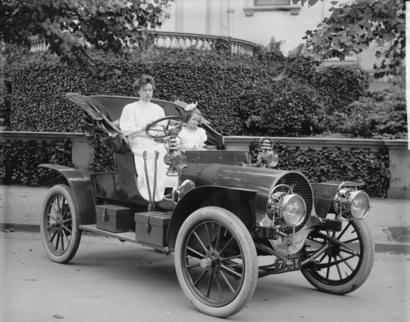
\includegraphics[width=\linewidth]{inc/sample-franklin}
%   \caption{1907 Franklin Model D roadster. Photograph by Harris \&
%     Ewing, Inc. [Public domain], via Wikimedia
%     Commons. (\url{https://goo.gl/VLCRBB}).}
%   \Description{A woman and a girl in white dresses sit in an open car.}
% \end{figure}

%% For a teaser figure.
% \begin{teaserfigure}
%   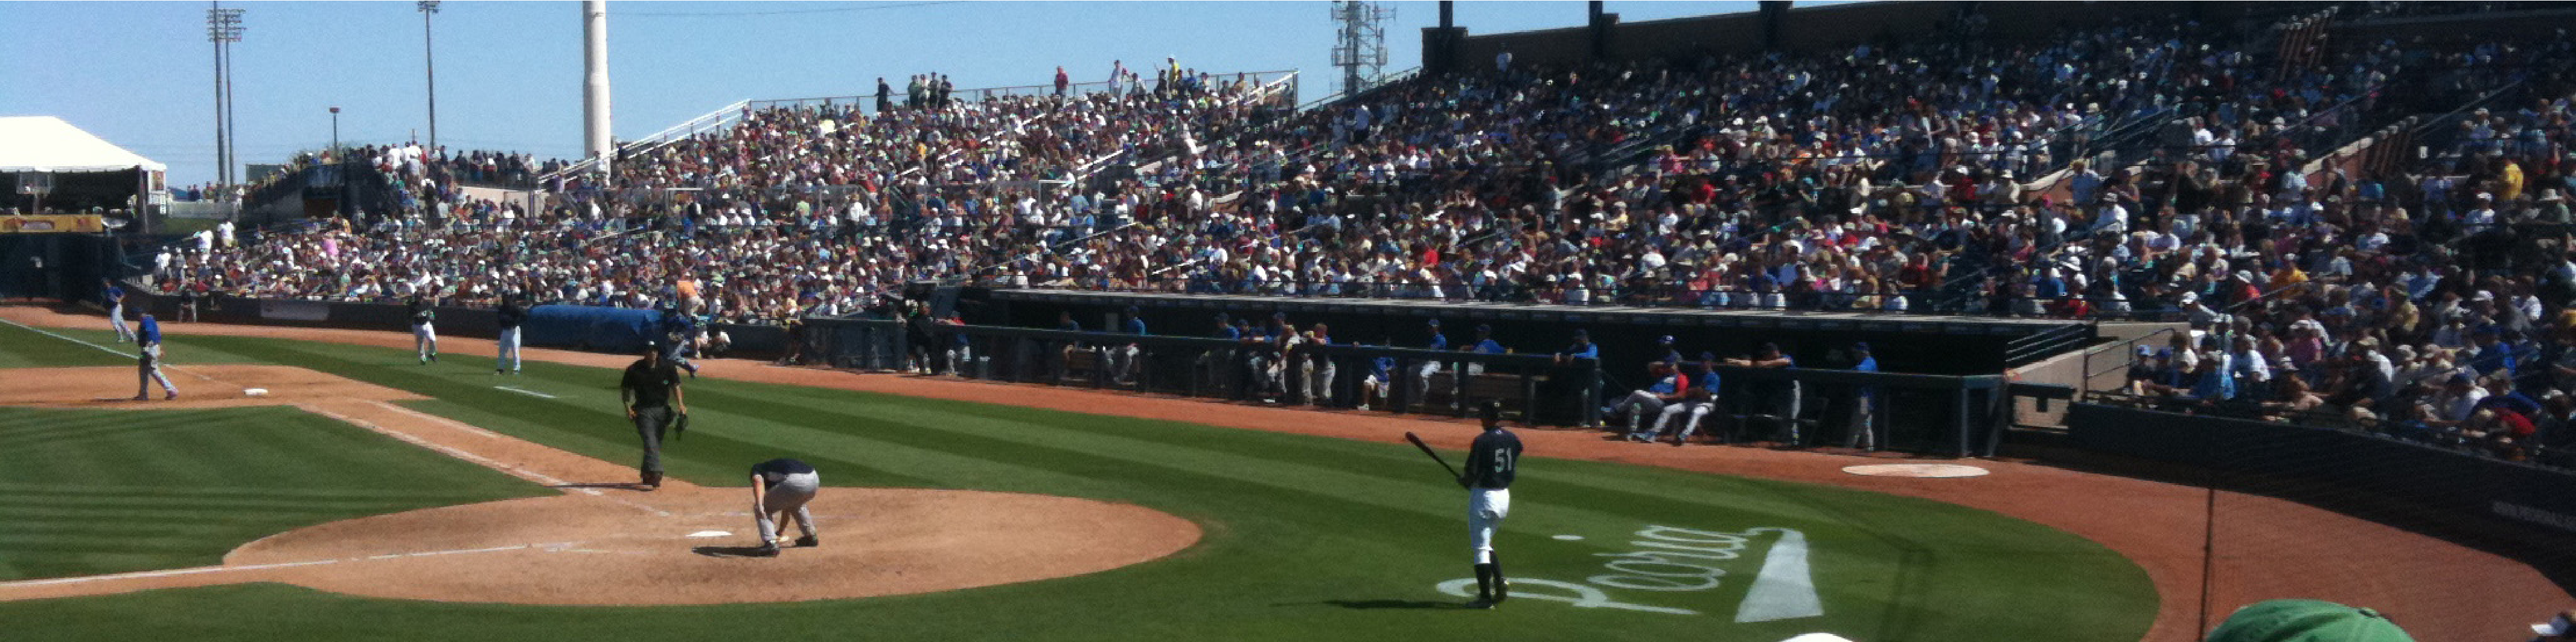
\includegraphics[width=\textwidth]{sampleteaser}
%   \caption{figure caption}
%   \Description{figure description}
% \end{teaserfigure}


\section{Related work}
\label{sec:related}
The \textit{Louvain} method is a greedy modularity-optimization based community detection algorithm \cite{com-blondel08}. It identifies communities with resulting high modularity, and is thus widely favored \cite{com-lancichinetti09}. Algorithmic improvements proposed for the original algorithm include early pruning of non-promising candidates (leaf vertices) \cite{com-ryu16, com-halappanavar17, com-zhang21, com-you22}, attempting local move only on likely vertices \cite{com-ryu16, com-ozaki16, com-zhang21, com-shi21}, ordering of vertices based on node importance \cite{com-aldabobi22}, moving nodes to a random neighbor community \cite{com-traag15}, threshold scaling \cite{com-lu15, com-naim17, com-halappanavar17}, threshold cycling \cite{com-ghosh18}, subnetwork refinement \cite{com-waltman13, com-traag19}, multilevel refinement \cite{com-rotta11, com-gach14, com-shi21}, and early termination \cite{com-ghosh18}.

To parallelize the Louvain algorithm, a number of strategies have been attempted. These include parallelizing the costly first iteration \cite{com-wickramaarachchi14}, performing iterations asynchronously \cite{com-que15, com-shi21}, ordering vertices via graph coloring \cite{com-halappanavar17}, using vector based hashtables \cite{com-halappanavar17}, using adaptive parallel thread assignment \cite{com-fazlali17, com-naim17, com-mohammadi20}, and using sort-reduce instead of hashing \cite{com-cheong13}\ignore{, using simple partitions based of vertex ids \cite{com-cheong13, com-ghosh18}, and identifying and moving ghost/doubtful vertices \cite{com-zeng15, com-que15, com-bhowmik19, com-bhowmick22}}.

The \textit{Label Propagation Algorithm (LPA)} is a diffusion-based technique for identifying communities. It is faster and more scalable than Louvain, as it does not require repeated optimization steps and is easier to parallelize \cite{com-newman04, com-raghavan07}. Improvements upon the LPA include using a stable (non-random) mechanism of label choosing in the case of multiple best labels \cite{com-xing14}, addressing the issue of monster communities \cite{com-berahmand18, com-sattari18}, identifying central nodes and combining communities for improved modularity \cite{com-you20}, and using frontiers with alternating push-pull to reduce the number of edges visited and improve solution quality \cite{com-liu20}.

A few open source implementations and software packages have been developed for community detection. Vite \cite{ghosh2018scalable} is a distributed memory parallel implementation of the Louvain method that incorporates several heuristics to enhance performance while maintaining solution quality, while Grappolo \cite{com-halappanavar17} is a shared memory parallel implementation. Fast Label Propagation Algorithm (FLPA) \cite{traag2023large} is a fast variant of the LPA, which utilizes a queue-based approach to process only vertices with recently updated neighborhoods. NetworKit \cite{staudt2016networkit} is a software package designed for analyzing the structural aspects of graph data sets with billions of connections. It is implemented as a hybrid with C++ kernels and a Python frontend, and includes parallel implementations of Louvain and LPA. igraph \cite{csardi2006igraph} is a similar package, written in C, with Python, R, and Mathematica frontends. It is widely used in academic research, and includes implementations of Louvain and LPA.


\section{Preliminaries}
\label{sec:preliminaries}
Consider an undirected graph $G(V, E, w)$ with $V$ representing the set of vertices, $E$ the set of edges, and $w_{ij} = w_{ji}$ denoting the weight associated with each edge. In the case of an unweighted graph, we assume unit weight for each edge ($w_{ij} = 1$). Additionally, the neighbors of a vertex $i$ are denoted as $J_i = \{j\ |\ (i, j) \in E\}$, the weighted degree of each vertex as $K_i = \sum_{j \in J_i} w_{ij}$, the total number of vertices as $N = |V|$, the total number of edges as $M = |E|$, and the sum of edge weights in the undirected graph as $m = \sum_{i, j \in V} w_{ij}/2$.




\subsection{Community detection}

Disjoint community detection is the process of identifying a community membership mapping, $C: V \rightarrow \Gamma$, where each vertex $i \in V$ is assigned a community-id $c \in \Gamma$, where $\Gamma$ is the set of community-ids. We denote the vertices of a community $c \in \Gamma$ as $V_c$, and the community that a vertex $i$ belongs to as $C_i$. Further, we denote the neighbors of vertex $i$ belonging to a community $c$ as $J_{i \rightarrow c} = \{j\ |\ j \in J_i\ and\ C_j = c\}$, the sum of those edge weights as $K_{i \rightarrow c} = \sum_{j \in J_{i \rightarrow c}} w_{ij}$, the sum of weights of edges within a community $c$ as $\sigma_c = \sum_{(i, j) \in E\ and\ C_i = C_j = c} w_{ij}$, and the total edge weight of a community $c$ as $\Sigma_c = \sum_{(i, j) \in E\ and\ C_i = c} w_{ij}$ \cite{com-leskovec21}.




\subsection{Modularity}

Modularity serves as a\ignore{fitness} metric for assessing the quality of communities identified by heuristic-based community detection algorithms. It is computed as the difference between the fraction of edges within communities and the expected fraction if edges were randomly distributed, yielding a range of $[-0.5, 1]$ where higher values indicate better results \cite{com-brandes07}.\ignore{The optimization of this metric theoretically leads to the optimal grouping \cite{com-newman04, com-traag11}.} The modularity $Q$ of identified communities is determined using Equation \ref{eq:modularity}, where $\delta$ represents the Kronecker delta function ($\delta (x,y)=1$ if $x=y$, $0$ otherwise). The \textit{delta modularity} of moving a vertex $i$ from community $d$ to community $c$, denoted as $\Delta Q_{i: d \rightarrow c}$, can be computed using Equation \ref{eq:delta-modularity}.

\begin{equation}
\label{eq:modularity}
  Q
  = \frac{1}{2m} \sum_{(i, j) \in E} \left[w_{ij} - \frac{K_i K_j}{2m}\right] \delta(C_i, C_j)
  = \sum_{c \in \Gamma} \left[\frac{\sigma_c}{2m} - \left(\frac{\Sigma_c}{2m}\right)^2\right]
\end{equation}

\begin{equation}
\label{eq:delta-modularity}
  \Delta Q_{i: d \rightarrow c}
  = \frac{1}{m} (K_{i \rightarrow c} - K_{i \rightarrow d}) - \frac{K_i}{2m^2} (K_i + \Sigma_c - \Sigma_d)
\end{equation}




\subsection{Louvain algorithm}
\label{sec:about-louvain}

The Louvain method \cite{com-blondel08} is a modularity optimization based agglomerative algorithm for identifying high quality disjoint communities in large networks. It has a time complexity of $O (L |E|)$ (with $L$ being the total number of iterations performed), and a space complexity of $O(|V| + |E|)$ \cite{com-lancichinetti09}. The algorithm consists of two phases: the \textit{local-moving phase}, where each vertex $i$ greedily decides to move to the community of one of its neighbors $j \in J_i$ that gives the greatest increase in modularity $\Delta Q_{i:C_i \rightarrow C_j}$ (using Equation \ref{eq:delta-modularity}), and the \textit{aggregation phase}, where all the vertices in a community are collapsed into a single super-vertex. These two phases make up one pass, which repeats until there is no further increase in modularity \cite{com-blondel08, com-leskovec21}. We observe that Louvain obtains high-quality communities, with $3.0 - 30\%$ higher modularity than that obtained by LPA, but requires $2.3 - 14\times$ longer to converge.


\section{Approach}
\label{sec:approach}
\subsection{Optimizations for Louvain algorithm}
\label{sec:louvain}

We use a parallel implementation of the Louvain method to determine suitable parameter settings and optimize the original algorithm through experimentation with a variety of techniques. We use \textit{asynchronous} version of Louvain, where threads work independently on different parts of the graph. This allows for faster convergence but can also lead to more variability in the final result \cite{com-blondel08, com-halappanavar17}. Further, we allocate a separate hashtable per thread to keep track of the delta-modularity of moving to each community linked to a vertex in the local-moving phase of the algorithm, and to keep track of the total edge weight from one super-vertex to the other super-vertices in the aggregation phase of the algorithm.

Our optimizations include using OpenMP's \verb|dynamic| loop schedule, limiting the number of iterations per pass to $20$, using a tolerance drop rate of $10$, setting an initial tolerance of $0.01$, using an aggregation tolerance of $0.8$, employing vertex pruning, making use of parallel prefix sum and preallocated Compressed Sparse Row (CSR) data structures for finding community vertices and for storing the super-vertex graph during the aggregation phase, and using fast collision-free per-thread hashtables which are well separated in their memory addresses (\textit{Far-KV}) for the local-moving and aggregation phases of the algorithm. Details\ignore{ on each of the optimizations is} are given below.

For each optimization, we test a number of relevant alternatives, and show the relative time and the relative modularity of communities obtained by each alternative in Figure \ref{fig:louvain-opt}. This result is obtained by running the tests on each graph in the dataset (see Table \ref{tab:dataset}), $5$ times on each graph to reduce the impact of noise, taking their geometric mean and arithmetic mean for the runtime and modularity respectively, and representing them as a ratio within each optimization category.


\subsubsection{Adjusting OpenMP loop schedule}

We attempt \textit{static}, \textit{dynamic}, \textit{guided}, and \textit{auto} loop scheduling approaches of OpenMP (each with a chunk size of $2048$) to parallelize the local-moving and aggregation phases of the Louvain algorithm. Results indicate that the scheduling behavior can have small impact on the quality of obtained communities. We consider OpenMP's \verb|dynamic| loop schedule to be the best choice, as it helps achieve better load balancing when the degree distribution of vertices is non-uniform, and offers a $7\%$ reduction in runtime with respect to OpenMP's \textit{auto} loop schedule, with only a $0.4\%$ reduction in the modularity of communities obtained (which is likely to be just noise).

\subsubsection{Limiting the number of iterations per pass}

Restricting the number of iterations of the local-moving phase ensures its termination within a reasonable number of iterations, which helps minimize runtime. This can be important since the local-moving phase performed in the first pass is the most expensive step of the algorithm. However, choosing too small a limit may worsen convergence rate. Our results indicate that limiting the maximum number of iterations to $20$ allows for $13\%$ faster convergence, when compared to a maximum iterations of $100$.


\subsubsection{Adjusting tolerance drop rate (threshold scaling)}

Tolerance is used to detect convergence in the local-moving phase of the Louvain algorithm, i.e., when the total delta-modularity in a given iteration is below or equal to the specified tolerance, the local-moving phase is considered to have converged. Instead of using a fixed tolerance across all passes of the Louvain algorithm, we can start with an initial high tolerance and then gradually reduce it. This is known as threshold scaling \cite{com-lu15, com-naim17, com-halappanavar17}, and it helps minimize runtime of the first pass of the algorithm (which is usually the most expensive). Based on our findings, a tolerance drop rate of $10$ yields $4\%$ faster convergence, with respect to a tolerance drop rate of $1$ (threshold scaling disabled), with no reduction in quality of communities obtained.


\subsubsection{Adjusting initial tolerance}

Starting with a smaller initial tolerance allows the algorithm to explore broader possibilities for community assignments in the early stage, but comes at the cost of increased runtime. We find an initial tolerance of $0.01$ provides a $14\%$ reduction in runtime of the algorithm with no reduction in the quality of identified communities, when compared to an initial tolerance of $10^{-6}$.


\subsubsection{Adjusting aggregation tolerance}

The aggregation tolerance determines the point at which communities are considered to have converged based on the number of community merges. In other words, if too few communities merged this pass we should stop here, i.e., if $|V_{aggregated}|/|V| \geq$ aggregation tolerance, we consider the algorithm to have converged. Adjusting aggregation tolerance allows the algorithm to stop earlier when further merges have minimal impact on the final result. According to our observations, an aggregation tolerance of $0.8$ appears to be the best choice, as it presents a $14\%$ reduction in runtime, when compared to the aggregation tolerance being disabled ($1$), while identifying final communities of equivalent quality.


\subsubsection{Vertex pruning}

Vertex pruning is a technique that is used to minimize unnecessary computation \cite{com-ryu16, com-ozaki16, com-zhang21, com-shi21}. Here, when a vertex changes its community, its marks its neighbors to be processed. Once a vertex has been processed, it is marked as not to be processed. However, it comes with an added overhead of marking an unmarking of vertices. Based on our results, vertex pruning justifies this overhead, and should be enabled for $11\%$ improvement in performance. An illustration of this\ignore{vertex pruning optimization} is shown in Figure \ref{fig:louvain-pruning}.

\begin{figure}[hbtp]
  \centering
  \subfigure{
    \label{fig:louvain-pruning--all}
    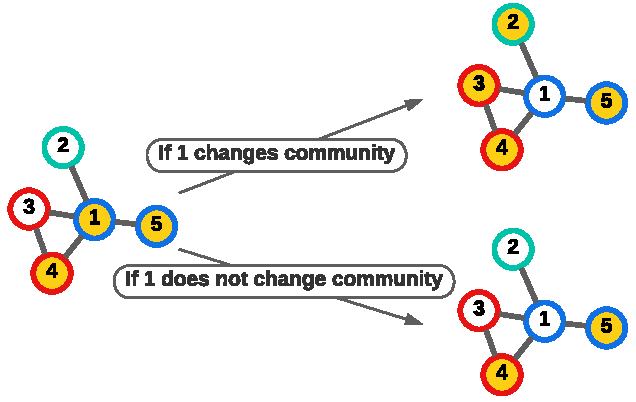
\includegraphics[width=0.78\linewidth]{out/louvain-pruning.pdf}
  } \\[-2ex]
  \caption{Illustration of vertex pruning optimization: After processing vertex $1$, it's unmarked. If vertex $1$ changes its community, its neighbors are marked for processing. Community membership of each vertex is depicted by border color, and marked vertices are highlighted in yellow.}
  \label{fig:louvain-pruning}
\end{figure}

\begin{figure}[hbtp]
  \centering
  \subfigure{
    \label{fig:louvain-hashtable--all}
    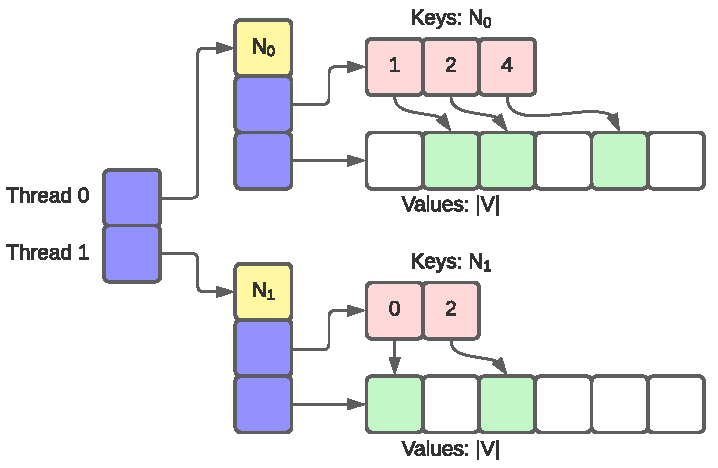
\includegraphics[width=0.88\linewidth]{out/louvain-hashtable.pdf}
  } \\[-2ex]
  \caption{Illustration of collision-free per-thread hashtables that are well separated in their memory addresses (Far-KV), for two threads. Each hashtable consists of a keys vector, values vector (of size $|V|$), and a key count ($N_0$/$N_1$). The value associated with each key is stored/accumulated in the index pointed by the key. As the key count of each hashtable is updated independently, we allocate it separately on the heap to avoid false cache sharing. These are used in the local-moving and aggregation phases of our Louvain implementation.}
  \label{fig:louvain-hashtable}
\end{figure}

\begin{figure*}[hbtp]
  \centering
  \subfigure{
    \label{fig:louvain-opt--all}
    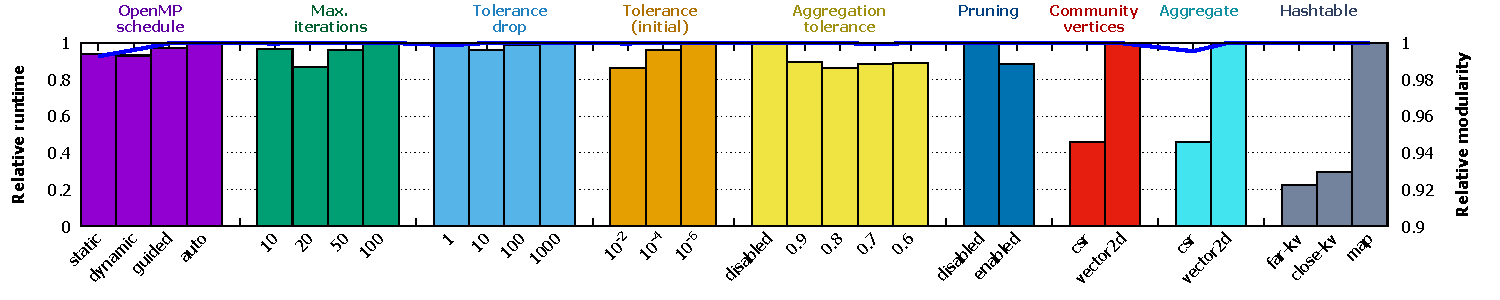
\includegraphics[width=0.98\linewidth]{out/louvain-opt.pdf}
  } \\[-2ex]
  \caption{Impact of various parameter controls and optimizations on the runtime and result quality (modularity) of the \Lou{} algorithm. We show the impact of each optimization upon the relative runtime on the left Y-axis, and upon the relative modularity on the right Y-axis.}
  \label{fig:louvain-opt}
\end{figure*}



\subsubsection{Finding community vertices for aggregation phase}

In the aggregation phase of the Louvain algorithm, the communities obtained in the previous local-moving phase of the algorithm are combined into super-vertices in the aggregated graph, with the edges between two super-vertices being equal to the total weight of edges between the respective communities. This requires one to obtain the list of vertices belonging to each community, instead of the mapping of community membership of each vertex that we have after the local-moving phase ends. A straight-forward implementation of this would make use of two-dimensional arrays for storing vertices belonging to each community, with the index in the first dimension representing the community id $c$, and the index in the second dimension pointing to the $n^{th}$ vertex in the given community $c$. However, this requires memory allocation during the algorithm, which is expensive. Employing a parallel prefix sum technique along with a preallocated Compressed Sparse Row (CSR) data structure eliminates repeated memory allocation and deallocation, enhancing performance. Indeed, out findings indicate that using parallel prefix sum along with a preallocated CSR is $2.2\times$ faster than using 2D arrays for aggregating vertices.


\subsubsection{Storing aggregated communities (super-vertex graph)}

After the list of vertices belonging to each community have been obtained, the communities need to be aggregated (or compressed) into super-vertices, such that edges between two super-vertices being equal to the total weight of edges between the respective communities. This is generally called the super-vertex graph, or the compressed graph. It is then used as an input to the local-moving phase of the next pass of the Louvain algorithm. A simple data structure to store the super-vertex graph in the adjacency list format would be a two-dimensional array. Again, this requires memory allocation during the algorithm, which is bad for performance. Utilizing two preallocated CSRs, one for the source graph and the other for the target graph (except the first pass, where the dynamic graph may be stored in any desired format suitable for dynamic batch updates), along with parallel prefix sum can help here. We observe that using parallel prefix sum along with preallocated CSRs for maintaining the super-vertex graph is again $2.2\times$ faster than using 2D arrays.


\subsubsection{Hashtable design for local-moving/aggregation phases}

One can use C++'s inbuilt maps as per-thread (independent) hashtables for the Louvain algorithm. But this has poor performance. So we use a key-list and a full-size values array (collision-free) to dramatically improve performance. However, if the memory addresses of the hashtables are nearby (\textit{Close-KV}) --- as with NetworKit Louvain \cite{staudt2016networkit}, even if each thread uses its own hashtable exclusively, performance is not as high. This is possibly due to false cache-sharing. Alternatively, if we ensure that the memory address of each hashtable are farther away (\textit{Far-KV}), the performance improves. Our results indicate that \textit{Far-KV} has the best performance and is $4.4\times$ faster than \textit{Map}, and $1.3\times$ faster than \textit{Close-KV} hashtable implementations. An illustration of \textit{Far-KV} hashtable is shown in Figure \ref{fig:louvain-hashtable}.




\subsection{Our optimized Louvain implementation}

We now explain the implementation of GVE-Louvain in Algorithms \ref{alg:louvain}, \ref{alg:louvainlm}, and \ref{alg:louvainag}. We aim to incorporate GVE-Louvain into our upcoming command-line graph processing tool named "GVE", derived from "Graph(Vertices, Edges)". GVE-Louvain exhibits a time complexity of $O(KM)$, where $K$ signifies the total iterations conducted. Its space complexity is $O(TN + M)$, where $T$ denotes the number of threads utilized, and $TN$ represents the collision-free hash tables $H_t$ employed per thread. A flow diagram illustrating the first pass of GVE-Louvain is shown in Figure \ref{fig:louvain-pass}.


\subsubsection{Main step of GVE-Louvain}

The main step of GVE-Louvain (\texttt{louvian()} function) is outlined in Algorithm \ref{alg:louvain}. It encompasses initialization, the local-moving phase, and the aggregation phase. Here, the \texttt{louvain()} function takes the input graph $G$, and returns the community membership $C$ for each vertex. In line \ref{alg:louvain--initialization}, we first initialize the community membership $C$ of each vertex in $G$, and perform passes of the Louvain algorithm, limited to $MAX\_PASSES$ (lines \ref{alg:louvain--passes-begin}-\ref{alg:louvain--passes-end}). In each pass, we initialize the total edge weight of each vertex $K'$, the total edge weight of each community $\Sigma'$, and the community membership $C'$ of each vertex in the current graph $G'$ (line \ref{alg:louvain--reset-weights}); and mark all vertices as unprocessed (line \ref{alg:louvain--reset-affected}).

\begin{algorithm}[hbtp]
\caption{GVE-Louvain: Our parallel Louvain algorithm.}
\label{alg:louvain}
\begin{algorithmic}[1]
\Require{$G$: Input graph}
\Require{$C$: Community membership of each vertex}
\Require{$G'$: Input/super-vertex graph}
\Require{$C'$: Community membership of each vertex in $G'$}
\Require{$K'$: Total edge weight of each vertex}
\Require{$\Sigma'$: Total edge weight of each community}
\Ensure{$G'_{C'}$: Community vertices (CSR)}
\Ensure{$H_t$: Collision-free per-thread hashtable}
\Ensure{$l_i$: Number of iterations performed (per pass)}
\Ensure{$l_p$: Number of passes performed}
\Ensure{$\tau$: Per iteration tolerance}
\Ensure{$\tau_{agg}$: Aggregation tolerance}

\Statex

\Function{louvain}{$G$} \label{alg:louvain--begin}
  \State Vertex membership: $C \gets [0 .. |V|)$ \textbf{;} $G' \gets G$ \label{alg:louvain--initialization}
  \ForAll{$l_p \in [0 .. \text{\small{MAX\_PASSES}})$} \label{alg:louvain--passes-begin}
    \State $\Sigma' \gets K' \gets vertexWeights(G')$ \textbf{;} $C' \gets [0 .. |V'|)$ \label{alg:louvain--reset-weights}
    \State Mark all vertices in $G'$ as unprocessed \label{alg:louvain--reset-affected}
    \State $l_i \gets louvainMove(G', C', K', \Sigma')$ \Comment{Alg. \ref{alg:louvainlm}} \label{alg:louvain--local-move}
    \If{$l_i \le 1$} \textbf{break} \Comment{Globally converged?} \label{alg:louvain--globally-converged}
    \EndIf
    \State $|\Gamma|, |\Gamma_{old}| \gets$ Number of communities in $C$, $C'$
    \If{$|\Gamma|/|\Gamma_{old}| > \tau_{agg}$} \textbf{break} \Comment{Low shrink?} \label{alg:louvain--aggregation-tolerance}
    \EndIf
    \State $C' \gets$ Renumber communities in $C'$ \label{alg:louvain--renumber}
    \State $C \gets$ Lookup dendrogram using $C$ to $C'$ \label{alg:louvain--lookup}
    \State $G' \gets louvainAggregate(G', C')$ \Comment{Alg. \ref{alg:louvainag}} \label{alg:louvain--aggregate}
    \State $\tau \gets \tau / \text{\small{TOLERANCE\_DROP}}$ \Comment{Threshold scaling} \label{alg:louvain--threshold-scaling}
  \EndFor \label{alg:louvain--passes-end}
  \State $C \gets$ Lookup dendrogram using $C$ to $C'$ \label{alg:louvain--lookup-last}
  \Return{$C$} \label{alg:louvain--return}
\EndFunction \label{alg:louvain--end}
\end{algorithmic}
\end{algorithm}

\begin{algorithm}[hbtp]
\caption{Local-moving phase of GVE-Louvain.}
\label{alg:louvainlm}
\begin{algorithmic}[1]
\Require{$G'$: Input/super-vertex graph}
\Require{$C'$: Community membership of each vertex}
\Require{$K'$: Total edge weight of each vertex}
\Require{$\Sigma'$: Total edge weight of each community}
\Ensure{$H_t$: Collision-free per-thread hashtable}
\Ensure{$l_i$: Number of iterations performed}
\Ensure{$\tau$: Per iteration tolerance}

\Statex

\Function{louvainMove}{$G', C', K', \Sigma'$} \label{alg:louvainlm--move-begin}
  \ForAll{$l_i \in [0 .. \text{\small{MAX\_ITERATIONS}})$} \label{alg:louvainlm--iterations-begin}
    \State Total delta-modularity per iteration: $\Delta Q \gets 0$ \label{alg:louvainlm--init-deltaq}
    \ForAll{unprocessed $i \in V'$ \textbf{in parallel}} \label{alg:louvainlm--loop-vertices-begin}
      \State Mark $i$ as processed (prune) \label{alg:louvainlm--prune}
      \State $H_t \gets scanCommunities(\{\}, G', C', i, false)$ \label{alg:louvainlm--scan}
      \State $\rhd$ Use $H_t, K', \Sigma'$ to choose best community
      \State $c^* \gets$ Best community linked to $i$ in $G'$ \label{alg:louvainlm--best-community-begin}
      \State $\delta Q^* \gets$ Delta-modularity of moving $i$ to $c^*$ \label{alg:louvainlm--best-community-end}
      \If{$c^* = C'[i]$} \textbf{continue} \label{alg:louvainlm--best-community-same}
      \EndIf
      \State $\Sigma'[C'[i]] -= K'[i]$ \textbf{;} $\Sigma'[c^*] += K'[i]$ \textbf{atomic} \label{alg:louvainlm--perform-move-begin}
      \State $C'[i] \gets c^*$ \textbf{;} $\Delta Q \gets \Delta Q + \delta Q^*$ \label{alg:louvainlm--perform-move-end}
      \State Mark neighbors of $i$ as unprocessed \label{alg:louvainlm--remark}
    \EndFor \label{alg:louvainlm--loop-vertices-end}
    \If{$\Delta Q \le \tau$} \textbf{break} \Comment{Locally converged?} \label{alg:louvainlm--locally-converged}
    \EndIf
  \EndFor \label{alg:louvainlm--iterations-end}
  \Return{$l_i$} \label{alg:louvainlm--return}
\EndFunction \label{alg:louvainlm--move-end}

\Statex

\Function{scanCommunities}{$H_t, G', C', i, self$}
  \ForAll{$(j, w) \in G'.edges(i)$}
    \If{\textbf{not} $self$ and $i = j$} \textbf{continue}
    \EndIf
    \State $H_t[C'[j]] \gets H_t[C'[j]] + w$
  \EndFor
  \Return{$H_t$}
\EndFunction
\end{algorithmic}
\end{algorithm}

\begin{algorithm}[hbtp]
\caption{Aggregation phase of GVE-Louvain.}
\label{alg:louvainag}
\begin{algorithmic}[1]
\Require{$G'$: Input/super-vertex graph}
\Require{$C'$: Community membership of each vertex}
\Ensure{$G'_{C'}$: Community vertices (CSR)}
\Ensure{$G''$: Super-vertex graph (weighted CSR)}
\Ensure{$*.offsets$: Offsets array of a CSR graph}
\Ensure{$H_t$: Collision-free per-thread hashtable}

\Statex

\Function{louvainAggregate}{$G', C'$}
  \State $\rhd$ Obtain vertices belonging to each community
  \State $G'_{C'}.offsets \gets countCommunityVertices(G', C')$ \label{alg:louvainag--coff-begin}
  \State $G'_{C'}.offsets \gets exclusiveScan(G'_{C'}.offsets)$ \label{alg:louvainag--coff-end}
  \ForAll{$i \in V'$ \textbf{in parallel}} \label{alg:louvainag--comv-begin}
    \State Add edge $(C'[i], i)$ to CSR $G'_{C'}$ atomically
  \EndFor \label{alg:louvainag--comv-end}
  \State $\rhd$ Obtain super-vertex graph
  \State $G''.offsets \gets communityTotalDegree(G', C')$ \label{alg:louvainag--yoff-begin}
  \State $G''.offsets \gets exclusiveScan(G''.offsets)$ \label{alg:louvainag--yoff-end}
  \State $|\Gamma| \gets$ Number of communities in $C'$
  \ForAll{$c \in [0, |\Gamma|)$ \textbf{in parallel}} \label{alg:louvainag--y-begin}
    \If{degree of $c$ in $G'_{C'} = 0$} \textbf{continue}
    \EndIf
    \State $H_t \gets \{\}$
    \ForAll{$i \in G'_{C'}.edges(c)$}
      \State $H_t \gets scanCommunities(H, G', C', i, true)$
    \EndFor
    \ForAll{$(d, w) \in H_t$}
      \State Add edge $(c, d, w)$ to CSR $G''$ atomically
    \EndFor
  \EndFor \label{alg:louvainag--y-end}
  \Return $G''$ \label{alg:louvainag--return}
\EndFunction
\end{algorithmic}
\end{algorithm}


Next, in line \ref{alg:louvain--local-move}, we perform the local-moving phase by calling \texttt{louvainMove()} (Algorithm $\ref{alg:louvainlm}$), which optimizes community assignments. If the local-moving phase converged in a single iteration, global convergence is implied and we terminate the passes (line \ref{alg:louvain--globally-converged}). Further, if the drop is community count $|\Gamma|$ is too small, we have reached the point of diminishing returns, and thus stop at the current pass (line \ref{alg:louvain--aggregation-tolerance}).

In case convergence has not been achieved, we renumber communities (line \ref{alg:louvain--renumber}), update top-level community memberships $C$ with dendrogram lookup (line \ref{alg:louvain--lookup}), perform the aggregation phase by calling \texttt{louvainAggregate()} (Algorithm \ref{alg:louvainag}), and scale the convergence threshold for subsequent passes, i.e., perform threshold scaling (line \ref{alg:louvain--threshold-scaling}). The next pass continues in line \ref{alg:louvain--passes-begin}. At the end of all passes, we perform a final update of the top-level community memberships $C$ with dendrogram lookup (line \ref{alg:louvain--lookup-last}), and return the top-level community membership $C$ of each vertex in $G$.


\subsubsection{Local-moving phase of GVE-Louvain}

The pseuodocode for the local-moving phase of GVE-Louvain is presented in Algorithm \ref{alg:louvainlm}, which iteratively moves vertices between communities to maximize modularity. Here, the \texttt{louvainMove()} function takes the current graph $G'$, community membership $C'$, total edge weight of each vertex $K'$, and total edge weight of each community $\Sigma'$ as input, and returns the number of iterations performed $l_i$.

Lines \ref{alg:louvainlm--iterations-begin}-\ref{alg:louvainlm--iterations-end} represent the main loop of the local-moving phase. In line \ref{alg:louvainlm--init-deltaq}, we first initialize the total delta-modularity per iteration $\Delta Q$. Next, in lines \ref{alg:louvainlm--loop-vertices-end}-\ref{alg:louvainlm--loop-vertices-end}, we iterate over unprocessed vertices in parallel. For each vertex $i$, we mark $i$ as processed - vertex pruning (line \ref{alg:louvainlm--prune}), scan communities connected to $i$ - excluding self (line \ref{alg:louvainlm--scan}), determine the best community $c*$ to move $i$ to (line \ref{alg:louvainlm--best-community-begin}), calculate the delta-modularity of moving $i$ to $c*$ (line \ref{alg:louvainlm--best-community-end}), and update the community membership  (lines \ref{alg:louvainlm--perform-move-begin}-\ref{alg:louvainlm--perform-move-end}) of $i$, and mark its neighbors as unprocessed (line \ref{alg:louvainlm--remark}) if a better community was found. In line \ref{alg:louvainlm--locally-converged}, we check if the local-moving phase has converged (locally). If so, we break out of the loop (or if $MAX\_ITERATIONS$ is reached). At the end, in line \ref{alg:louvainlm--return}, we return the number of iterations performed $l_i$.


\subsubsection{Aggregation phase of GVE-Louvain}

Finally, the psuedocode for the aggregation phase is shown in Algorithm \ref{alg:louvainag}, which aggregates communities into super-vertices. Here, the \texttt{louvainAggrega} \texttt{te()} function takes the current graph $G'$ and the community membership $C'$ as input, and returns the super-vertex graph $G''$.

In lines \ref{alg:louvainag--coff-begin}-\ref{alg:louvainag--coff-end}, the offsets array for the community vertices CSR $G'_{C'}.offsets$ is obtained by first counting the number of vertices belonging to each community using \texttt{countCommunity} \texttt{Vertices()}, and then performing exclusive scan on the array. In lines \ref{alg:louvainag--comv-begin}-\ref{alg:louvainag--comv-end}, we iterate over all vertices in parallel and atomically populate vertices belonging to each community into the community graph CSR $G'_{C'}$. Next, we obtain the offsets array for the super-vertex graph CSR by over-estimating the degree of each super-vertex, i.e., by obtaining the total degree of each community with \texttt{communityTotalDegree()}, and then performing exclusive scan on the array (lines \ref{alg:louvainag--yoff-begin}-\ref{alg:louvainag--yoff-end}). This causes the super-vertex graph CSR to be holey, i.e., with gaps in between the edges and weights array of each super-vertex in the CSR. Then, in lines \ref{alg:louvainag--y-begin}-\ref{alg:louvainag--y-end}, we iterate over all communities $c \in [0, |\Gamma|)$ in parallel, and add all communities $d$ (with associated edge weight $w$) linked to each vertex $i$ belonging to community $c$ (with \texttt{scanCommunities()} defined in Algorithm \ref{alg:louvainlm}) to the per-thread hashtable $H_t$. Once $H_t$ is populated with all communities (and associated weights) linked to community $c$, we add them as edges to super-vertex $c$ into the super-vertex graph $G''$ atomically. At the end, in line \ref{alg:louvainag--return}, we return the super-vertex graph $G''$.

\ignore{The main Louvain algorithm, given in Algorithm \ref{alg:louvain} first initializes the community membership of each vertex. It then iteratively performs the local-moving phase until convergence. In each pass, it resets the edge weights, marks vertices as unprocessed, and performs the local-moving phase. If the algorithm globally converges or the communities' shrinkage is below a specified tolerance, it breaks the loop. Otherwise, it renumbers the communities, updates the graph, and adjusts the convergence threshold. The main algorithm returns the final community membership of each vertex.}

\ignore{The local-moving phase is responsible for iteratively moving vertices between communities to maximize modularity. It uses a per-thread hashtable to keep track of the communities and their weights. The algorithm iterates over unprocessed vertices, scans their neighbors, and identifies the best community for each vertex based on delta-modularity. If the best community is different from the current community, it updates the community memberships and marks neighbors as unprocessed. The process continues until a specified number of iterations or until local convergence is achieved.}

\ignore{The aggregation phase aggregates communities into super-vertices to reduce the size of the graph. It first counts the vertices in each community and constructs a new graph with community vertices. It then calculates the total degree of each community and constructs a super-vertex graph. The algorithm ensures that only communities with a non-zero degree are considered. It utilizes a per-thread hashtable to efficiently aggregate edges between communities. The resulting super-vertex graph is returned to the main algorithm for the next iteration.}

\begin{figure*}[hbtp]
  \centering
  \subfigure{
    \label{fig:louvain-pass--all}
    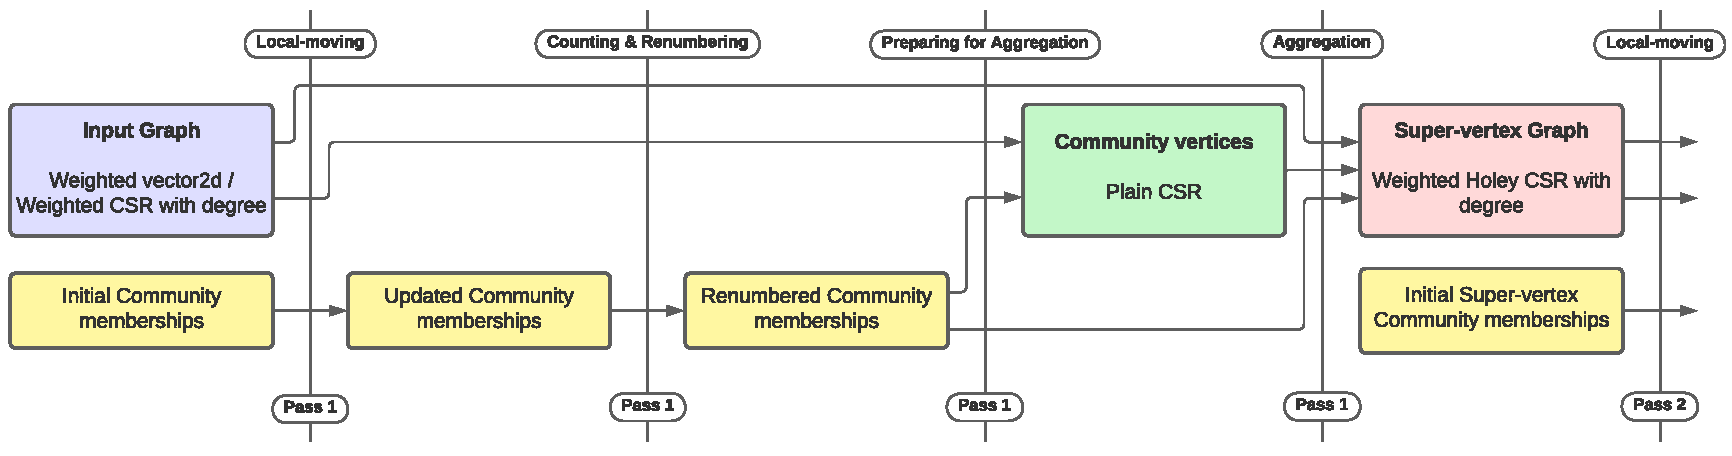
\includegraphics[width=0.98\linewidth]{out/louvain-pass.pdf}
  } \\[-2ex]
  \caption{A flow diagram illustrating the first pass of GVE-Louvain for a Weighted 2D-vector based or a Weighted CSR with degree based input graph. In the local-moving phase, vertex community memberships are updated until the total change in delta-modularity across all vertices reaches a specified threshold. Community memberships are then counted and renumbered. In the aggregation phase, community vertices in a CSR are first obtained. This is used to create the super-vertex graph stored in a Weighted Holey CSR with degree. In subsequent passes, the input is a Weighted Holey CSR with degree and initial community membership for super-vertices from the previous pass.}
  \label{fig:louvain-pass}
\end{figure*}
% A flow diagram showing the high level steps followed in the first pass of our Louvain implementation. The input graph is a weighted 2D vector based graph or weighted CSR with degree graph. In the local-moving phase, the community membership of each vertex is updated until the net change in delta-modularity across all vertices in an iteration reaches a threshold/tolerance. The community memberships are then counted and renumbered. In the aggregation phase of the algorithm, we obtain the vertices belonging to each community as a CSR, and later use this to generate the super-vertex graph. The super-vertex graph is stored in a weighted holey CSR with degree, i.e., the CSR is over-allocated with gaps between edges (ids and weights), and a degree vector is instead used to keep track of the degree of each super-vertex. In the remaining passes, the input graph is a weighted holey CSR with degree (from the previous pass) and an initial community membership vector for each super-vertex.


\section{Evaluation}
\label{sec:evaluation}
\subsection{Experimental Setup}
\label{sec:setup}

We use a server that has two $16$-core x86-based Intel Xeon Gold 6226R processors running at $2.90$ GHz. Each core has an L1 cache of $1$ MB, an L2 cache of $16$ MB, and a shared L3 cache of $22$ MB. The machine has $93.4$ GB of system memory and runs on CentOS Stream 8. We use GCC 8.5 and OpenMP 4.5. Table \ref{tab:dataset} shows the graphs we use in our experiments. All of them are obtained from the SuiteSparse Matrix Collection \cite{suite19}.

\begin{table}[hbtp]
  \centering
  \caption{List of $13$ graphs obtained SuiteSparse Matrix Collection \cite{suite19} (directed graphs are marked with $*$). Here, $|V|$ is the number of vertices, $|E|$ is the number of edges (after adding reverse edges), $D_{avg}$ is the average degree, and $|\Gamma|$ is the number of communities obtained using Louvain algorithm.\ignore{In the table, B refers to a billion, M refers to a million and K refers a thousand.}}
  \label{tab:dataset}
  \begin{tabular}{|c||c|c|c|c|}
    \toprule
    \textbf{Graph} &
    \textbf{\textbf{$|V|$}} &
    \textbf{\textbf{$|E|$}} &
    \textbf{\textbf{$D_{avg}$}} &
    \textbf{\textbf{$|\Gamma|$}} \\
    % \textbf{$1 - \Gamma_G$} \\
    \midrule
    \multicolumn{5}{|c|}{\textbf{Web Graphs (LAW)}} \\ \hline
    indochina-2004$^*$ & 7.41M & 341M & 41.0 & 4.24K \\ \hline  % & \num{4.7e-4} & 2.9 GB
    uk-2002$^*$ & 18.5M & 567M & 16.1 & 42.8K \\ \hline  % & \num{9.6e-5} & 16 GB
    arabic-2005$^*$ & 22.7M & 1.21B & 28.2 & 3.66K \\ \hline  % & \num{5.5e-4} & 11 GB
    uk-2005$^*$ & 39.5M & 1.73B & 23.7 & 20.8K \\ \hline  % & \num{9.6e-5} & 16 GB
    webbase-2001$^*$ & 118M & 1.89B & 8.6 & 2.76M \\ \hline  % & \num{7.3e-7} & 18 GB
    it-2004$^*$ & 41.3M & 2.19B & 27.9 & 5.28K \\ \hline  % & \num{3.8e-4} & 19 GB
    sk-2005$^*$ & 50.6M & 3.80B & 38.5 & 3.47K \\ \hline  % & \num{5.8e-4} & 33 GB
    \multicolumn{5}{|c|}{\textbf{Social Networks (SNAP)}} \\ \hline
    com-LiveJournal & 4.00M & 69.4M & 17.4 & 2.54K \\ \hline  % & \num{7.9e-4} & 480 MB
    com-Orkut & 3.07M & 234M & 76.2 & 29 \\ \hline  % & \num{6.7e-2} & 1.7 GB
    \multicolumn{5}{|c|}{\textbf{Road Networks (DIMACS10)}} \\ \hline
    asia\_osm & 12.0M & 25.4M & 2.1 & 2.38K \\ \hline  % & \num{8.4e-4} & 200 MB
    europe\_osm & 50.9M & 108M & 2.1 & 3.05K \\ \hline  % & \num{6.6e-4} & 910 MB
    \multicolumn{5}{|c|}{\textbf{Protein k-mer Graphs (GenBank)}} \\ \hline
    kmer\_A2a & 171M & 361M & 2.1 & 21.2K \\ \hline  % & \num{9.4e-5} & 3.2 GB
    kmer\_V1r & 214M & 465M & 2.2 & 6.17K \\ \hline  % & \num{3.2e-4} & 4.2 GB
  \bottomrule
  \end{tabular}
\end{table}
% We convert directed graphs (marked with $*$) to undirected by duplicating edges in the reverse direction, and set the weight of each edge to $1$. and $F_{size}$ is size of the \textit{MatrixMarket} file

\begin{figure*}[hbtp]
  \centering
  \subfigure{
    \label{fig:louvain-compare--all}
    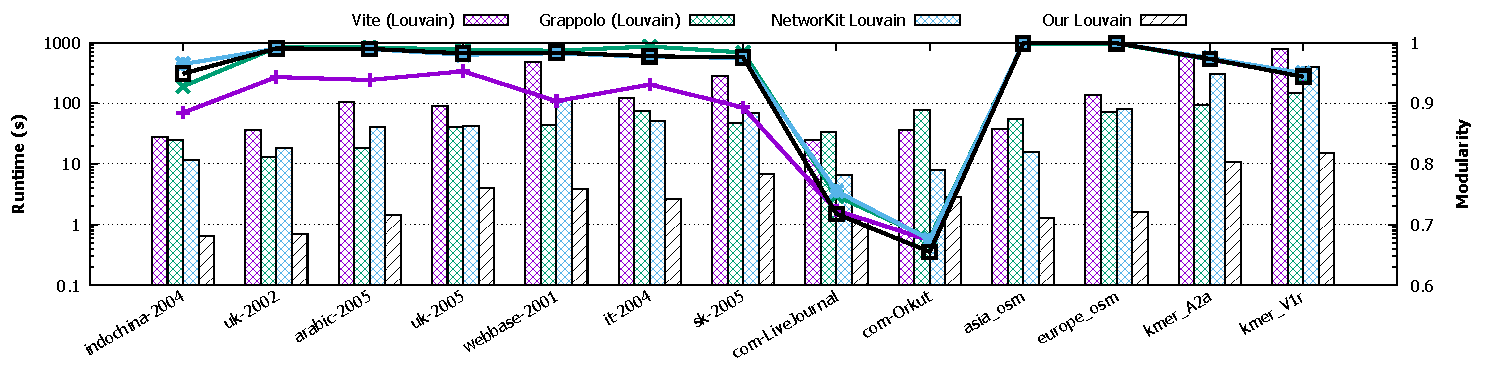
\includegraphics[width=0.98\linewidth]{out/louvain-compare.pdf}
  } \\[-2ex]
  \caption{Time taken (boxes), and modularity of communities obtained (lines) with \textit{Vite}, \textit{Grappolo}, \textit{NetworKit}, and our \textit{Louvain} for each graph in the dataset. Runtime is shown with logarithmic scale on the left Y-axis (in seconds), and modularity is shown with linear scale on the right Y-axis.}
  \label{fig:louvain-compare}
\end{figure*}

\begin{figure*}[hbtp]
  \centering
  \subfigure{
    \label{fig:louvain-compares--all}
    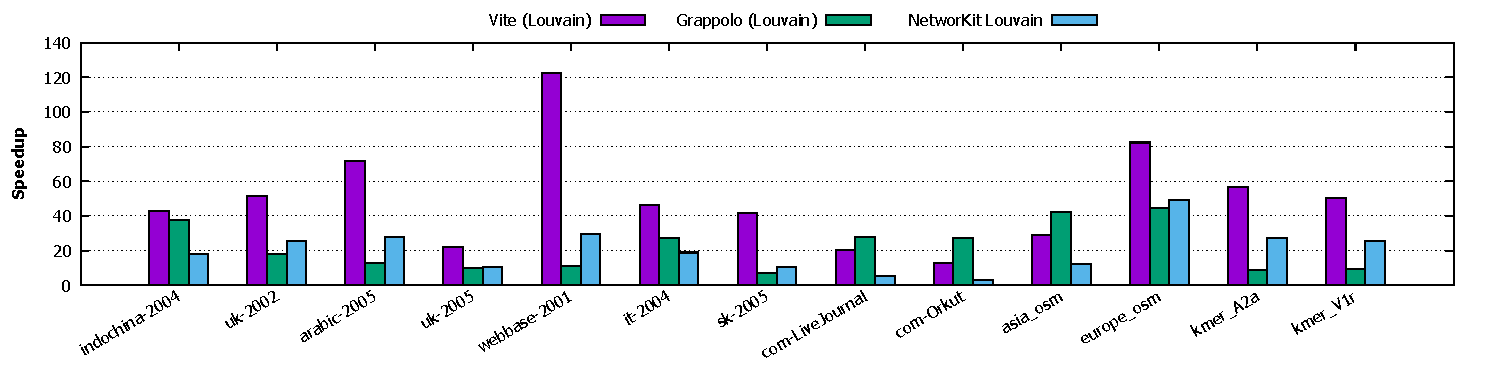
\includegraphics[width=0.98\linewidth]{out/louvain-compares.pdf}
  } \\[-2ex]
  \caption{Speedup of our \textit{Louvain} with respect to \textit{Vite}, \textit{Grappolo}, and \textit{NetworKit} for each graph in the dataset.}
  \label{fig:louvain-compares}
\end{figure*}

\begin{figure*}[hbtp]
  \centering
  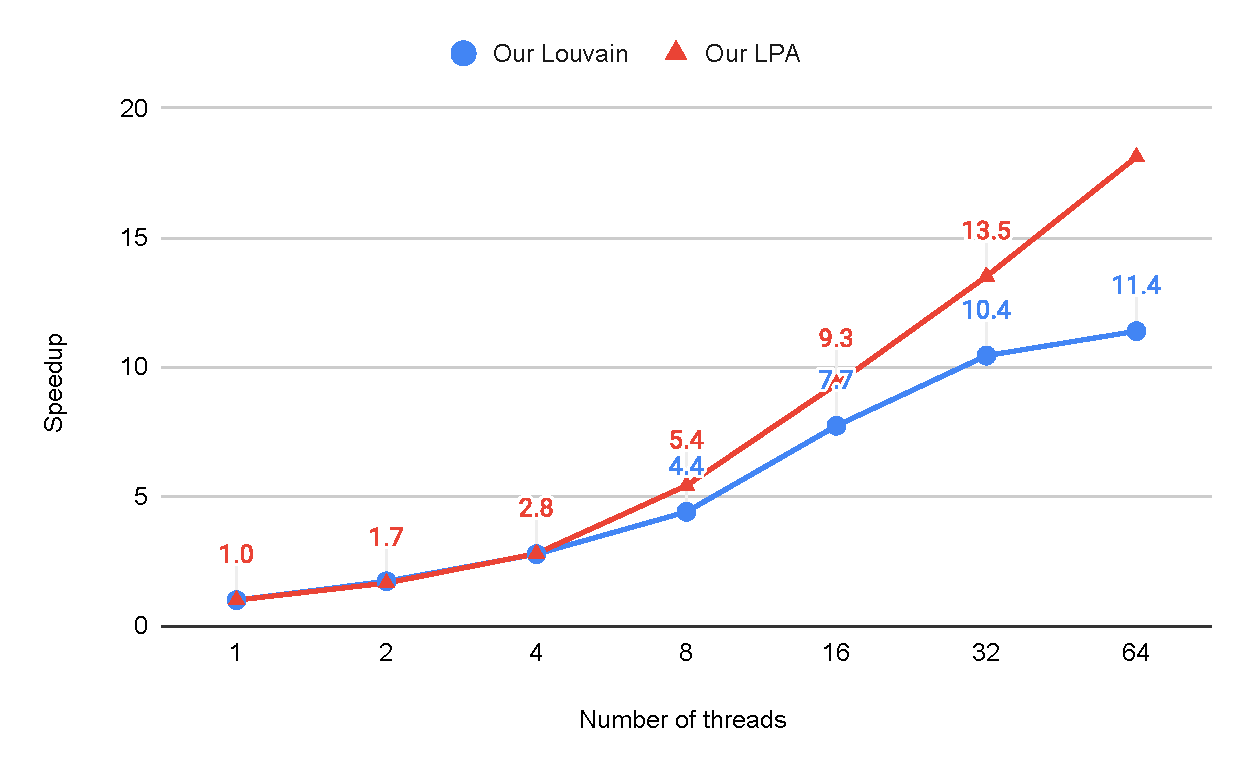
\includegraphics[width=0.68\linewidth]{out/louvain-ss.pdf} \\[-2ex]
  \caption{Speedup of our \textit{Louvain} with increasing number of threads.}
  \label{fig:louvain-ss}
\end{figure*}





\subsection{Comparing Performance of GVE-Louvain}

We now compare the performance of GVE-Louvain with Vite (Louvain), Grappolo (Louvain), and NetworKit Louvain. For Vite, we convert the graph datasets to Vite's binary graph format, run it on a single node (Vite supports distributed community detection) with threshold cycling/scaling optimization, and measure the reported average total time. For Grappolo, we measure the run it on the same system, and measure the reported total time. For NetworKit, we use a Python script to invoke \texttt{PLM} (Parallel Louvain Method), and measure the total time reported with \texttt{getTiming()}. For each graph, we measure the runtime of each implementation five times, for averaging. We also record the modularity of communities obtained, as reported by each implementation.

Figure \ref{fig:louvain-compare} shows the runtimes of Vite (Louvain), Grappolo (Louvain), NetworKit Louvain, and GVE-Louvain on each graph in the dataset. Figure \ref{fig:louvain-compares} shows the speedup of GVE-Louvain with respect to each implementation mentioned above. GVE-Louvain is on average $50\times$, $22\times$, and $20\times$ faster than Vite, Grappolo, and NetworKit respectively. On the \textit{sk-2005} graph, GVE-Louvain finds communities in $6.8$ seconds, and thus achieve a processing rate of $560$ million edges/s. Figure \ref{fig:louvain-compare} also shows the modularity of communities obtained with each implementation on the secondary (right) Y-axis. GVE-Louvain on average obtains $3.1\%$ higher modularity than Vite (especially on web graph), and $0.6\%$ lower modularity than Grappolo and NetworKit (especially on social networks with poor clustering).

\begin{figure*}[hbtp]
  \centering
  \subfigure{
    \label{fig:louvain-hardness--all}
    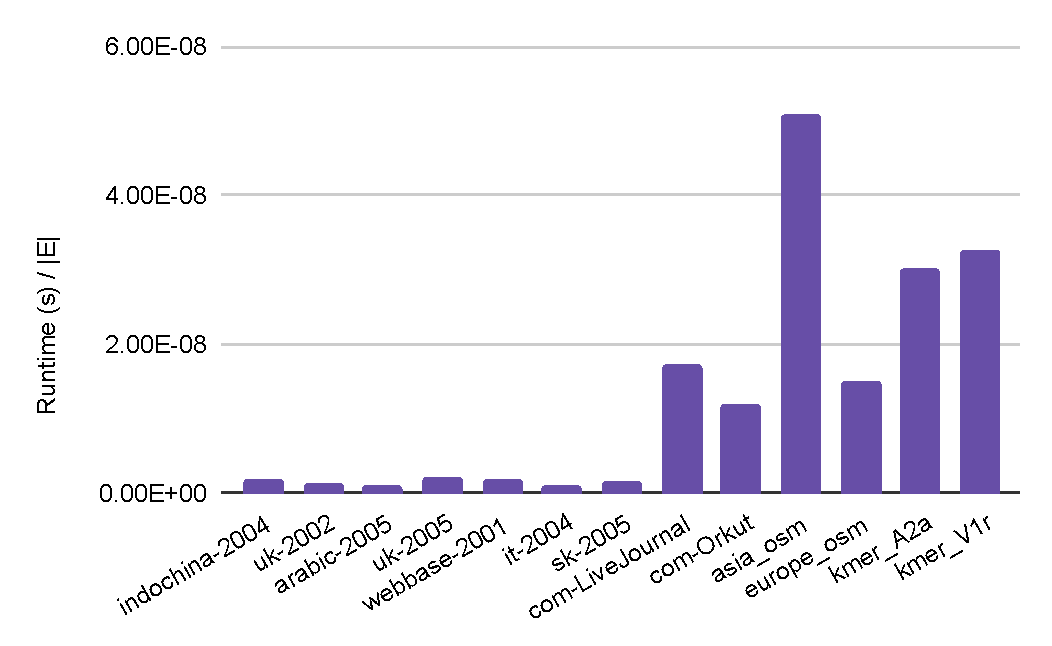
\includegraphics[width=0.48\linewidth]{out/louvain-hardness.pdf}
  } \\[-2ex]
  \caption{Runtime $/ |E|$ with our \textit{Louvain}, showing ...}
  \label{fig:louvain-hardness}
\end{figure*}

\begin{figure*}[hbtp]
  \centering
  \subfigure[Phase split]{
    \label{fig:louvain-splits--phase}
    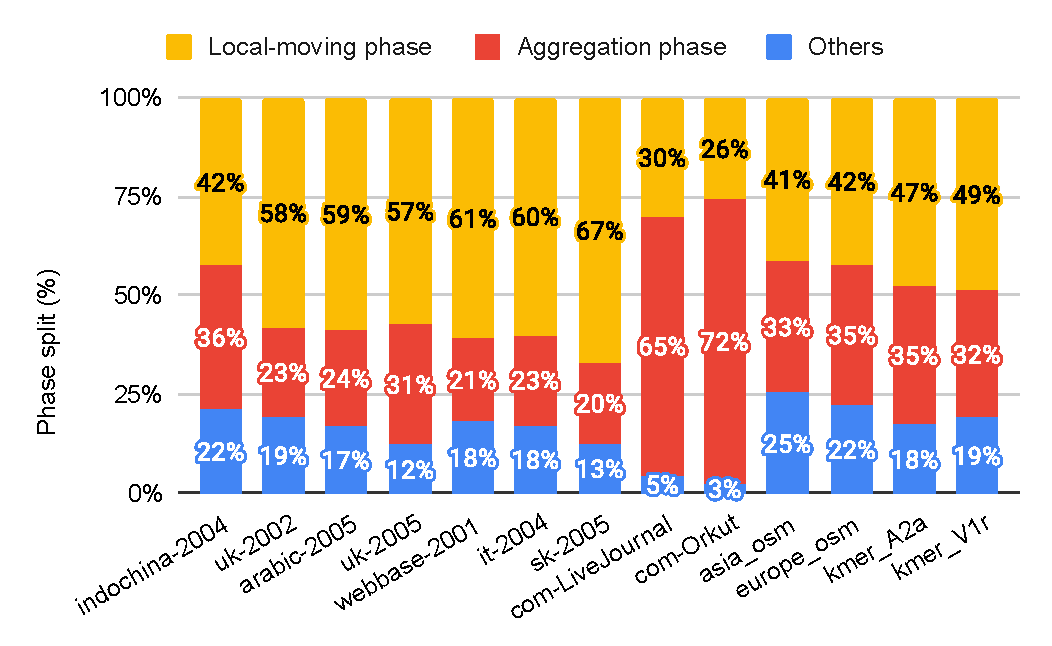
\includegraphics[width=0.48\linewidth]{out/louvain-phases.pdf}
  }
  \subfigure[Pass split]{
    \label{fig:louvain-splits--pass}
    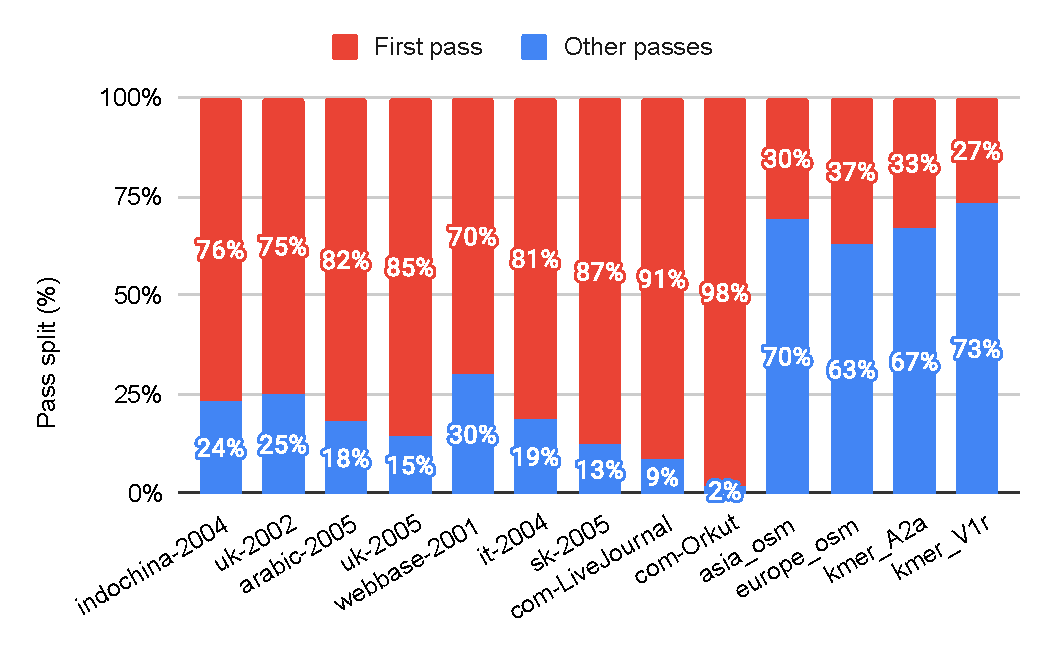
\includegraphics[width=0.48\linewidth]{out/louvain-passes.pdf}
  } \\[-2ex]
  \caption{Phase split of \textit{GVE-Louvain} shown on the left, and pass split shown on the right for each graph in the dataset.}
  \label{fig:louvain-splits}
\end{figure*}





\subsection{Results with our optimized implementation}

The combined optimizations yield impressive performance improvements in the OpenMP-based \StaLou{}, with a completion time of $6.8$ seconds on the \textit{sk-2005} graph containing $3.8 B$ edges (refer to Figure \ref{fig:louvainrak-sta}). We observe that graphs with lower average degree (\textit{road networks} and \textit{protein k-mer graphs}) and graphs with poor community structure (such as \verb|com-LiveJournal| and \verb|com-Orkut|) have a larger $\text{runtime}/|E|$ factor, as shown in Figure \ref{fig:louvainrak-hardness--louvain}.

The phase-wise and pass-wise split of the optimized \StaLou{} is shown in Figure \ref{fig:louvain-splits}. Note how $48\%$ (most) of the runtime of the algorithm is spent in the local-moving phase, while only $29\%$ of the runtime is spent in the aggregation phase of the algorithm. Further, $68\%$ (most) of the runtime is spent in the first pass of the algorithm, which is the most expensive pass due to the size of the original graph (later passes work on super-vertex graphs) \cite{com-wickramaarachchi14}.




\subsection{Strong Scaling of GVECD}

Finally, we measure the strong scaling performance of our Louvain and LPA. To this end, we adjust the number of thread from $1$ to $64$ in multiples of $2$ for each input graph, and measure the time taken for finding communities within each graph with our Louvain and LPA. As for each experiment above, for each graph, and for each thread count, we perform our Louvain and LPA five times for averaging. The results are shown in Figure \ref{fig:louvainrak-ss}. With 32 threads, finding communities with our Louvain obtains a $10.4\times$ speedup compared to running with a single thread, i.e., the performance of our Louvain increases by $1.6\times$ for every doubling of threads. Further, with 32 threads, finding communities with our LPA obtains a speedup of $13.5\times$ with respect to a single threaded execution, i.e., our LPA's performance increases by $1.7\times$ for every doubling of threads. Our LPA is thus more scalable than our Louvain due to its algorithmic simplicity (one only phase, in contrast to Louvain which has both a local-moving and an aggregation phase along with an expensive initialization step). At 64 threads, both our Louvain and our LPA are impacted by NUMA effects, and offer speedups of only $11.4\times$ and $18.1\times$ respectively. Note that our Louvain is significantly affected due to the reasons mentioned above.


\section{Conclusion}
\label{sec:conclusion}
In conclusion, this report presents our parallel multicore implementation of the Louvain algorithm --- a high quality community detection method, which, as far as we are aware, stands as the most efficient implementation of the algorithm on multicore CPUs. Here, we considered $9$ different optimizations, which significantly improve the performance of the local-moving and the aggregation phases of the algorithm. On a server with dual 16-core Intel Xeon Gold 6226R processors, comparison with competitive open source implementations (Vite and Grappolo) and packages (NetworKit) show that our optimized implementation of Louvain, which we term as GVE-Louvain, is on average $50\times$, $22\times$, and $20\times$ faster than Vite, Grappolo, and NetworKit respectively. In addition, GVE-Louvain on average obtains $3.1\%$ higher modularity than Vite\ignore{(especially on web graph)}, and $0.6\%$ lower modularity than Grappolo and NetworKit\ignore{(especially on social networks with poor clustering)}. On a web graph with $3.8$ billion edges, GVE-Louvain identifies communities in $6.8$ seconds, and thus achieves a processing rate of $560$ million edges/s. In addition, GVE-Louvain achieves a strong scaling factor of $1.6\times$ for every doubling of threads. Looking ahead, future work could focus of designing dynamic algorithms for Louvain to accommodate dynamic graphs which evolve over time.\ignore{This would contribute to interactive updation of community memberships of vertices in real-world scenarios.}


%% The acknowledgments section.
\begin{acks}
I would like to thank Prof. Kishore Kothapalli,  Prof. Dip Sankar Banerjee, Balavarun Pedapudi, Souvik Karfa, Chuck Hastings, and Rick Ratzel for their support.
\end{acks}

%% Bibliography style to be used, and the bibliography file.
\bibliographystyle{ACM-Reference-Format}
\bibliography{main}

\clearpage
\appendix
\section{Appendix}
\subsection{Indirect Comparison with State-of-the-art Louvain Implementations}
\label{sec:comparison-indirect}

We now indirectly compare the performance of our multicore implementation of Louvain algorithm with other similar state-of-the-art implementations, listed in Table \ref{tab:compare}. Mohammadi et al. \cite{com-mohammadi20} propose the Adaptive CUDA Louvain Method (ACLM), employing GPU acceleration. Their approach involves evaluating the change in modularity for each edge in the graph, reflecting the impact of moving the source vertex to the community of the target vertex. Notably, only the computation of modularity changes occurs on the GPU, with other algorithmic steps executed on the CPU. For a computational setup featuring a $12$-core AMD Opteron 6344 CPU clocked at $2.60$ GHz alongside an NVIDIA Tesla K20Xm GPU, Mohammadi et al. report a runtime of $0.47$ seconds for ACLM when applied to the \textit{in-2004} graph with $13.6$ million edges (refer to Table 6 in \cite{com-mohammadi20}). Moreover, they document runtimes of $3.71$, $0.60$, and $0.95$ seconds for PLM \cite{staudt2015engineering}, APLM \cite{com-fazlali17}, and Rundemanen \cite{com-naim17} respectively (also presented in Table 6 of \cite{com-mohammadi20}). In contrast, leveraging our system equipped with two $16$-core Intel Xeon Gold 6226R CPUs operating at $2.90$ GHz (delivering up to $3.0\times$ higher performance), we process the \textit{indochina-2004} graph boasting $341$ million edges ($25.1\times$ larger) in merely $0.65$ seconds. Consequently, our Louvain implementation outperforms ACLM, PLM, APLM, and Rundemanen by approximately $6.0\times$, $48\times$, $7.7\times$, and $12.2\times$ respectively, all\ignore{achieved} without a GPU.

Sattar and Arifuzzaman \cite{sattar2022scalable} discuss their Distributed Parallel Louvain Algorithm with Load-balancing (DPLAL). They begin by partitioning the input graph using METIS, employing the edge-cut partitioning approach. In each iteration, they determine the optimal community to relocate to for each vertex, execute community changes while tackling duality concerns, evaluate the new modularity, and generate the subsequent level graph. This iterative process continues until no further enhancement in modularity is achieved. Nonetheless, they conduct only a single iteration of the local-moving phase per iteration, which might result in the identification of substandard quality communities.\ignore{It is not clear if they perform local-moves to the best community per vertex, or just any community with a positive delta-modularity score. They do not present the quality of returned communities.} On a graph containing $1M$ vertices, utilizing $40$ compute nodes of the Louisiana Optical Network Infrastructure (LONI) QB2 cluster, where each node is equipped with two $10$ core $2.80$ GHz Intel Xeon E5-2680v2 CPUs, they achieve community detection within approximately $80$ seconds (refer to Figure 4 in their paper \cite{sattar2022scalable}). In contrast, employing our system\ignore{featuring two $16$ core Intel Xeon Gold 6226R CPUs operating at $2.90$ GHz} (which is $6.0\times$ slower, assuming DPLAL utilizes each node with only $25\%$ efficiency), we process the \textit{indochina-2004} graph with $7.41M$ vertices ($7.41\times$ larger) in only $0.65$ seconds. Consequently, our Louvain implementation is roughly $5472\times$ faster\ignore{ than DPLAL}\ignore{ exhibits a speedup of roughly $5472\times$ compared to DPLAL}.

Qie et al. \cite{qie2022isolate} present a graph partitioning algorithm that divides the graph into sets of partitions, aiming to minimize inter-partition communication delay and avoid community swaps, akin to the graph coloring approach proposed by Halappanavar et al. \cite{com-halappanavar17}. We do not observe community swap issue on CPUs (it likely resolves itself), but do observe it on GPUs (likely due to lockstep execution). Their experiments on an $8$ core Intel i9 9900K CPU running at $3.60$ GHz, using the \textit{com-LiveJournal} graph, reveal a runtime of approximately $1050$ seconds (as depicted in Figure 3 of their paper \cite{qie2022isolate}). In contrast, on our system\ignore{ leveraging our system equipped with two $16$ core Intel Xeon Gold 6226R CPUs running at $2.90$ GHz} (roughly $3.2\times$ faster), we process the same graph in merely $1.2$ seconds. Consequently, our Louvain implementation achieves a speedup of about $273\times$.

Bhowmick et al. \cite{com-bhowmik19} introduce HyDetect, a community detection algorithm designed for hybrid CPU-GPU systems, employing a divide-and-conquer strategy. The algorithm partitions the graph among the CPU and GPU components of a node, facilitating independent community detection utilizing the Louvain algorithm in both segments. Their experimentation on a system comprising a six-core Intel Xeon E5-2620 CPU operating at $2.00$ GHz paired with an NVIDIA Kepler K40M GPU yields a runtime of $1123$ seconds when applied to the \textit{it-2004} graph (as documented in Table 5 of their paper \cite{com-bhowmik19}). In contrast, leveraging our system equipped with two $16$ core Intel Xeon Gold 6226R CPUs running at $2.90$ GHz (approximately $7.7\times$ faster), we process the same graph in $2.7$ seconds. Consequently, our Louvain implementation achieves a speedup of around $54\times$ compared to HyDetect, without using a GPU.

Bhowmick et al. \cite{com-bhowmick22} later introduce a multi-node multi-GPU Louvain community detection algorithm, which involves graph partitioning across multiple nodes, refinement through identification and migration of doubtful vertices between processors, and utilization of a hierarchical merging algorithm ensuring that the merged components can be accommodated within a processor at any given point. Their experimentation conducted on a CrayXC40 system, where each node comprises one $12$ core $2.40$ GHz Intel Xeon Ivybridge E5-2695 v2 CPU and one NVIDIA Tesla K40 GPU, demonstrates the capability to identify communities within approximately $32$ seconds on the \textit{uk-2005} graph utilizing $8$ compute nodes (refer to Figure 8 in their paper \cite{com-bhowmick22}). Furthermore, they observe a speedup of about $1.7\times$ compared to Cheong et al. \cite{com-cheong13} on the \textit{uk-2005} graph (as depicted in Figure 11 of their paper), and a speedup of approximately $1.2\times$ relative to Ghost et al. \cite{com-ghosh18} on the \textit{sk-2005} graph (as shown in Figure 10 of their paper). In contrast, on our system featuring two $16$ core Intel Xeon Gold 6226R CPUs operating at $2.90$ GHz (up to $1.6\times$ faster, assuming Bhowmick et al. utilize each compute node with only $25\%$ efficiency), we process the \textit{uk-2005} graph in a mere $4.1$ seconds. Thus, our Louvain implementation achieves at least $4.9\times$, $8.3\times$, and $5.9\times$ speedup compared to Multi-node HyDetect \cite{com-bhowmick22}, Cheong et al. \cite{com-cheong13}, and Ghost et al. \cite{com-ghosh18}, respectively, without requiring the use of a single GPU.

Chou and Ghosh \cite{chou2022batched} present Nido, a batched clustering method for GPUs that leverages a partition-based design, and can process graphs larger than the combined GPU memory of a node. Their experimentation conducted on a system equipped with two $128$ core AMD EPYC 7742 CPUs running at $2.25$ GHz and eight NVIDIA A100 GPUs demonstrates a (geometric) mean speedup of $2.4\times$ compared to Grappolo \cite{com-halappanavar17}, utilizing $128$ threads (as shown in Table 3 of their paper \cite{chou2022batched}). Additionally, they find that cuGraph \cite{hricik2020using} offers a mean speedup of $7.7\times$ relative to Grappolo (also depicted in Table 3 of their paper). In contrast, our Louvain implementation achieves a mean speedup of $22\times$ compared to Grappolo. Consequently, it surpasses Chou and Ghosh by $9.2\times$ and cuGraph by $2.9\times$\ignore{, without employing a single GPU}.

Gawande et al. \cite{com-gawande22} propose cuVite, an ongoing endeavor focusing on distributed Louvain for heterogeneous systems --- building upon their previous work involving parallelizing the Louvain method for community detection on CPU-only distributed systems. They evaluate cuVite, cuGraph, and Rundemanen on a single-GPU of NVIDIA DGX-2, i.e., NVIDIA Tesla V100, and with two $24$ core Intel Xeon Platinum 8168 CPUs running at $2.7$ GHz. Further, they evaluate Grappolo on a $224$ core system with eight $28$ core Intel Xeon Platinum 8276M CPUs running at $2.20$ GHz. They observe that, on average, cuGraph, Rundemanen, and cuVite exhibit speedups of $3.3\times$, $3.0\times$, and $3.28\times$ respectively compared to Grappolo. \ignore{Further analysis on the \textit{webbase-2001} graph indicates that cuVite (32 nodes) achieves a speedup of $1.3\times$ (including remapping) or $2.0\times$ faster (excluding remapping) relative to Grappolo (128 threads), while Vite (32 nodes) demonstrates a speedup of 2.3 times. Notably, cuVite does not significantly outperform Vite, and in some cases, it exhibits slower performance.} Consequently, our Louvain implementation achieves a speedup of $6.7\times$ compared to both cuGraph and cuVite, and a speedup of $7.3\times$ relative to Rundemanen, all achieved without the utilization of a GPU.

\end{document}
\endinput
%% End of file.
